\subsection{Dijkstra's Algorithm}

The first solution proposed in this thesis is a modified version of Dijkstra's algorithm, which is a well-known algorithm for finding the shortest path between two vertices in a weighted graph. The algorithm works by selecting the node with the smallest distance from the source node and updating the distance of its neighbors. This process is repeated until all vertices have been visited. The algorithm is efficient for finding the shortest path between two vertices in a graph with non-negative edge weights. However, it is not suitable for graphs with negative edge weights.

Adapting the methodogies used by Pezzica et al. \cite{cormen2022introduction}, which incooperate the Dijkstra's algorithm with a (Minimum) Priority Queue data structure. The data structure maintains a dynamic set $S$ of elements, each set element in $S$ has a key and it supports the following dynamic-set operations.

\begin{itemize}
    \item INSERT($S; x; k$): inserts element $x$ with key $k$ into set $S$.
    \item MINIMUM($S$): returns element of $S$ with smallest key.
    \item EXTRACT-MIN($S$): removes and returns element of $S$ with smallest key.
    \item DECREASE-KEY($S;x;k$): decreases value of element $x$’s key to $k$. Assumes $k\leq x$’s current key value.
\end{itemize}

All operations take $O(\log n)$ time in an $n$-element heap with the exception of $\text{MINIMUM}(S)$ being $\Theta(1)$.

We extend the algorithm so that the algotithm will stop once all nodes within $t$ minutes have been visited. As the 15-Minute City concept is primarily used to study cities' characteristics, the input graph of the algorithm is expected to be far larger than each 15 minute area. Therefore, it is necessary to stop the algorithm once all nodes within $t$ minutes have been visited to prevent the algorithm from running indefinitely. The modified algorithm is shown in Algorithm \ref{alg:modified_dijsktra}.

\begin{algorithm}[H]
    \caption{ModifiedDijkstra Algorithm} \label{alg:modified_dijsktra}
    \textbf{Input:} A graph $G(V,E)$, weights $w:E\rightarrow\mathbb{R}_{\geq 0}$, source vertex $s$, \\ \phantom{\textbf{Input:}} time threshold $t$ and $i$ denotes the index of the service type\\
    \textbf{Output} Assign $v.r[i]=1$ for vertices that can reach to source node $s$ within threshold $t$ % Set $S$ of vertices reachable by at most $t$ minutes
    \begin{algorithmic}
        \For {each vertex $v\in V$}
            \State $v.d\gets\infty$
        \EndFor
        \State $s.d\gets 0$
        % \State $S\gets\emptyset$
        \State $Q\gets\emptyset$
        \For {each vertex $v\in V$}
            \State INSERT($Q,v$)
        \EndFor
        \While {$Q\neq\emptyset$}
            \State $v\gets$EXTRACT-MIN$(Q)$
            \If {$v.d>t$}
                \State $Q\gets\emptyset$ \Comment{Break out of While loop}
            \Else
                % \State $S\gets S\cup\{v\}$
                \State $v.r[i] \gets 1 $
                \For {each vertex $u\in Adj[v]$}
                    \If {$u.d>v.d+w(u,v)$}
                        \State $u.d\gets v.d+w(u,v)$
                        \State DECREASE-KEY($Q,u,u.d$)
                    \EndIf
                \EndFor
            \EndIf
        \EndWhile
    \end{algorithmic}
\end{algorithm}

The modified Dijkstra's algorithm shown above only searches for vertices within $t$ minutes from a single source node. For our context of the 15-Minute City, this needs to run for each location of each service type. The full algorithm as the solution of the problem is shown in Algorithm \ref{alg:15mc}.

\begin{algorithm}[H]
    \caption{15-Minute City Algorithm}\label{alg:15mc}
    \textbf{Input:} A graph $G(V,E)$, weights $w:E\rightarrow\mathbb{R}_{\geq 0}$, a time threshold $t$ \\ \phantom{\textbf{Input:}} and a list $S$ of service vertices of $n$ types\\
    \textbf{Output} Set $R\subseteq V$ representing the $t$-Minute City
    \begin{algorithmic}
        \ForAll{vertex $v \in V$}
            \State $v.r \gets \{\mathbf{0}\}^{n}$
            \State $v.l \gets 0$
        \EndFor
        \ForAll{service $v \in S$}
            \State $v.l \gets i^{th}$ type of service
        \EndFor
        \For {each service type $i\in\{1,...,n\}$}
            % \State $S\gets\emptyset$
            \For {each vertex $s$ where $s.l=i$}
                \State $\text{ModifiedDijkstra}(G,w,s,t,i)$
                % \State $S\gets S\cup\text{ModifiedDijkstra}(G,w,s,t,i)$
            \EndFor
            % \For {each vertex $v\in S$}
            %     \State $v.r[i] \gets 1$
            % \EndFor
        \EndFor
        \State $R\gets\emptyset$
        \For {each vertex $v\in V$}
            \If {$v.r = \mathbf{1}$}
                \State $R \gets R\cup \{v\}$
            \EndIf
        \EndFor
    \end{algorithmic}
\end{algorithm}

\subsubsection{Analysis}

The time complexity of the modified Dijkstra's algorithm depends on the following:

\begin{itemize}
    \item Initialisation: $O(V)$
    \item $\text{INSERT}$: $|V|\cdot O(|\text{INSERT}|)=O(|V|\cdot|\text{INSERT}|)$
    \item $\text{EXTRACT-MIN}$: $|V|\cdot O(|\text{EXTRACT-MIN}|)=O(|V|\cdot|\text{EXTRACT-MIN}|)$
    \item $\text{DECREASE-KEY}$: $|E|\cdot O(|\text{DECREASE-KEY}|)=O(|E|\cdot|\text{DECREASE-KEY}|)$
\end{itemize}

The time complexity of the algorithm is also affected by the data structure used to implement the priority queue. A binary heap is a common choice for implementing a priority queue, which has a time complexity of $O(\log V)$ for $\text{INSERT}$, $\text{EXTRACT-MIN}$ and $\text{DECREASE-KEY}$ operations. However, if a Fibonacci heap is used instead, the time complexity of the operations is reduced to $O(1)$, $O(\log V)$ and $O(1)$ respectively.

As the latter two operations in the algorithm dominates the former two operations, the time complexity of algorithm \ref{alg:modified_dijsktra} is $O((V+E)\log V)$ if a binary heap is implemented. This can be reduced to $O(V\log V+E)$ if a Fibonacci heap is considered instead.

For the complete 15-Minute City Algorithm \ref{alg:15mc}, the algorithm is run for each location of each service type. Denote $m$ as the maximum number of locations for any service type, the time complexity of the algorithm is $O(n\cdot m\cdot(V\log V+E))$ if a binary heap is implemented and $O(n\cdot m\cdot(V\log V+E))$ if a Fibonacci heap is implemented. 

In both cases, the time complexity consider the size of the entire graph, which could be arbitrarily large when a city or a large area is studied. Due to the fact that the modified dijsktra's algorithm stops once all nodes within weight $t$ are searched, it is important to note that the actual complexity of the algorithm is much smaller. For example, consider a city with only square grids and each edge has a weight of 1 (see image \ref{fig:grid_city}) The algorithm will effectively only search a total of 100 edges and 141 nodes.

\begin{figure}[h]
    \caption{Example of grid city}
    \centering
    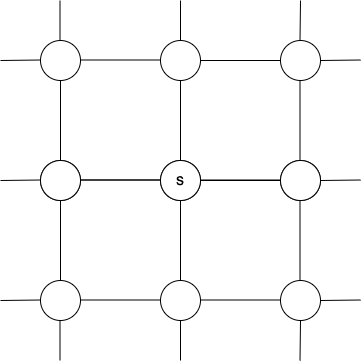
\includegraphics[width=0.5\textwidth]{grid_city.png}
    \label{fig:grid_city}
\end{figure}

However, if the graph of interest has the following characteristics: starting from the source node $s$, each node expands the graph with 4 edges of weight 1. (An illustration of the graph with 2 levels are shown in figure \ref{fig:tree_city}) In this arrangment, given a parameter level $l$, the number of nodes and edges can be calculated as follows:

$$|\text{Edges}|=\sum^{15}_{l=0}4^{l-1},\enspace|\text{Vertices}|=\sum^{15}_{l=1}4^{l-1}$$

Consider the case where a level in this calculation represents a minute of travelling time, the modified dijsktra's algorithm will have a time complexity with $|E|=357913941$ and $|V|=1431655765$.

\begin{figure}[h]
    \caption{Example of a tree city at 2 levels}
    \centering
    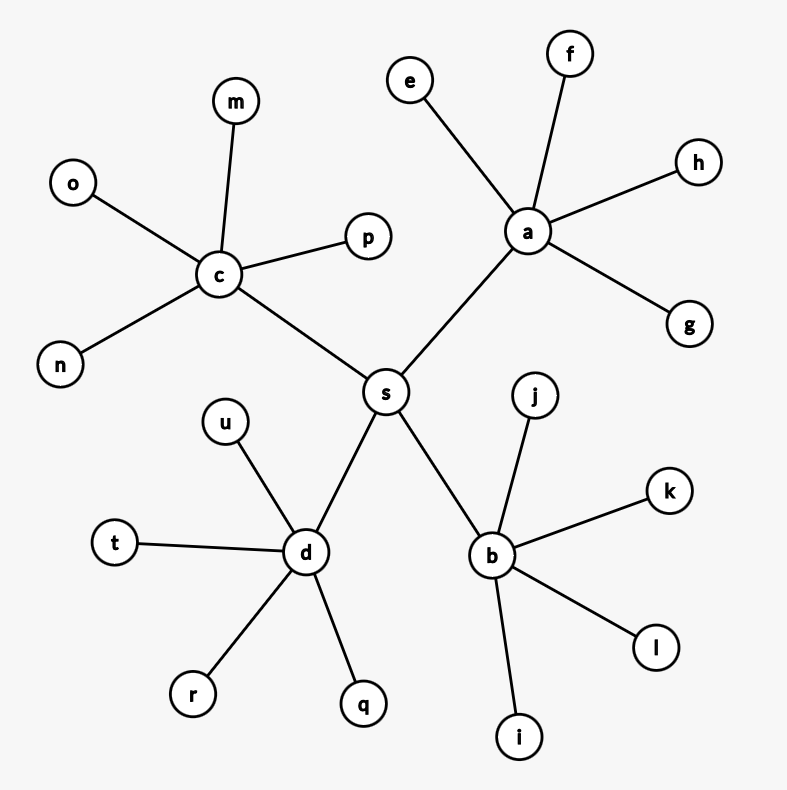
\includegraphics[width=0.5\textwidth]{tree_city.png}
    \label{fig:tree_city}
\end{figure}

\subsection{Dijkstra's Algorithm Revisit}

The second version of the algorithm proposed aims to improve on the complexity of the first version, the algorithm searches from multiple source nodes simultaneously. Therefore, this algorithm will allow us to find all vertices that can reach to a location of a specific service type within $t$ minutes. The algorithm is shown in Algorithm %\ref{alg:15mc_revisit}.

\subsection{All Pairs Shortest Path}

